\documentclass[12pt]{article}
\usepackage{hyperref}
\usepackage{listings}
\usepackage[margin=1in]{geometry}
\usepackage{enumitem}
\usepackage{multicol}
\usepackage{array}
\usepackage{titlesec}
\usepackage{helvet}
\renewcommand{\familydefault}{\sfdefault}
\usepackage{amsmath}     % For math equations
\usepackage{amssymb}     % For advanced math symbols
\usepackage{amsfonts} % For math fonts
\usepackage{gvv}
\usepackage{esint}
\usepackage[utf8]{inputenc}
\usepackage{graphicx}
\usepackage{pgfplots}
\pgfplotsset{compat=1.18}
\titleformat{\section}{\bfseries\large}{\thesection.}{1em}{}
\setlength{\parindent}{0pt}
\setlength{\parskip}{6pt}
\usepackage{multirow}
\usepackage{float}
\usepackage{caption}


\begin{document}
\section*{Problem 3.4.1}
Draw a quadrilateral in the Cartesian plane, whose vertices are
$A(-4,5)$, $B(0,7)$, $C(5,-5)$ and $D(-4,-2)$.

\subsection*{Solution}
The position vectors of the vertices are
\begin{align}
\vec{A} &= \myvec{-4\\5}, \\
\vec{B} &= \myvec{0\\7}, \\
\vec{C} &= \myvec{5\\-5}, \\
\vec{D} &= \myvec{-4\\-2}.
\end{align}

\begin{figure}[H]
    \centering
    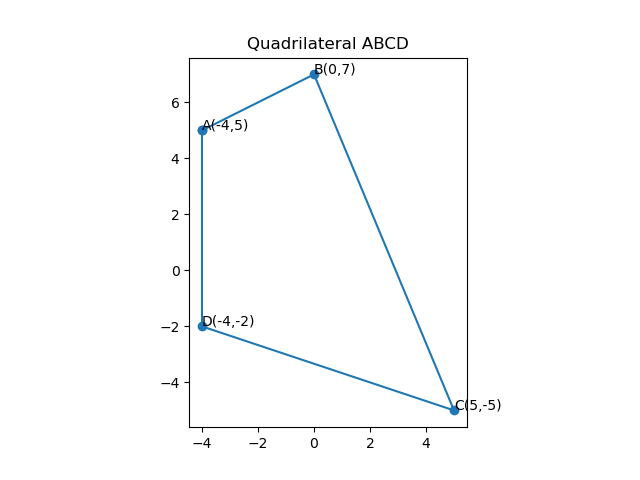
\includegraphics[width=0.9\columnwidth]{figs/quad_only.png}
    \caption{}
    \label{fig:placeholder}
\end{figure}



\end{document}
